%%%%%%%%%%%%%%%%%%%%
%%%% Formatting and UDFs %%%%%
%%%%%%%%%%%%%%%%%%%%

% Set page spacing
\documentclass[twoside, 11pt-]{article}
\usepackage[utf8]{inputenc}
\setlength{\oddsidemargin}{0.25 in}
\setlength{\evensidemargin}{-0.25 in}
\setlength{\topmargin}{-0.6 in}
\setlength{\textwidth}{6.5 in}
\setlength{\textheight}{8.5 in}
\setlength{\headsep}{0.75 in}
\setlength{\parindent}{0 in}
\setlength{\parskip}{0.1 in}

% Imports
\usepackage{amsmath,amsfonts,graphicx, hyperref, listings, color, titlesec, enumitem}

% formatting the subsection fonts
\titleformat*{\subsection}{\normalsize\bfseries}

% for clickable table of contents
\hypersetup{colorlinks, citecolor=black, filecolor=black, linkcolor=black, urlcolor=black}

% set parameters for the way that code blocks look
\definecolor{gray}{rgb}{0.5, 0.5, 0.5}
\lstset{frame = tb,
	language=Matlab,
	aboveskip=3mm,
	belowskip=3mm,
	showstringspaces=false,
	columns=flexible,
	basicstyle={\small\ttfamily},
	numbers=none,
	numberstyle=\tiny\color{red},
	keywordstyle=\color{blue},
	commentstyle=\color{gray},
	stringstyle=\color{red},
	breaklines=true,
	breakatwhitespace=true,
	tabsize=3
}

% Makes Table of Contents say Summary instead of Contents
\renewcommand*\contentsname{Summary}

%%%%%%%%%%%%%%%%%%%%%%%%%%%%%%%%%%%%%%


\title{\bf{Machine Learning}}
\author{Andrew Ng}
\date{}


\begin{document}

\maketitle \thispagestyle{empty}
\tableofcontents \newpage


\section{Machine Learning in a Nutshell}


\subsection{Supervized vs Unsupervized Learning}

\textbf{Supervised Learning} problems are typically regressions and classification problems. These problems aim to find a way to make the most correct predictions. To do this, you have to define criteria for "correct" and the program will iteratively take an enormous number of stabs to find an equation that returns the most correct predictions.

\textbf{Unsupervised Learning} are things like clustering and recommender systems. These algorithms objectively group similar datapoints without any specific instruction in order to higlight patterns that naturally occur in the data.

\subsection{General Form of Regression and Cost Functions}

\begin{center}
	\begin{tabular}{l c l}
		\multicolumn{3}{c}{Notation}\\\hline
		\textbf{m}: The number of training examples & & \textbf{X}: Input variables / features \\
		\textbf{y}: Output variable / target & & \textbf{h}: hypothesis, mapping \textbf{X} to \textbf{y} \\
		(x, y) : one training example & & ($x^{(i)}, y^{(i)}$) : the $i^{th}$ training example
	\end{tabular}
\end{center}


Generally speaking, for supervised learning algorithms the cost function fits the form
\[ h_\Theta (x) = \Theta_0 + \Theta_1 x\]
where $\Theta_0$ is a given and then we multiply $\Theta_1$ by $x$ to get the total cost value. Our supervised learning algorithm adjusts the $\Theta$'s (taking the values for $x$ as given) until $h_\Theta$ looks like we want it to.

We want to choose our $\Theta$'s so as to most accurately predict our $y$'s, thus minimizing the distance between the predictions and our observations.

In math, we call this the \emph{Squared Error Function}:
\[J(\Theta_0, \Theta_1) = \frac{1}{2m} \sum_{i = 1}^{m} (h_\Theta (x^{(i)}) - y^{(i)})^2\]
\vspace{-1cm}
\[\min_{\Theta_0, \Theta_1} J(\Theta_0, \Theta_1)\]

\subsection{Gradient Descent}

Graphically, our Squared Error Function looks like a hyperplane with a huge sink in the center

\begin{figure}[h]
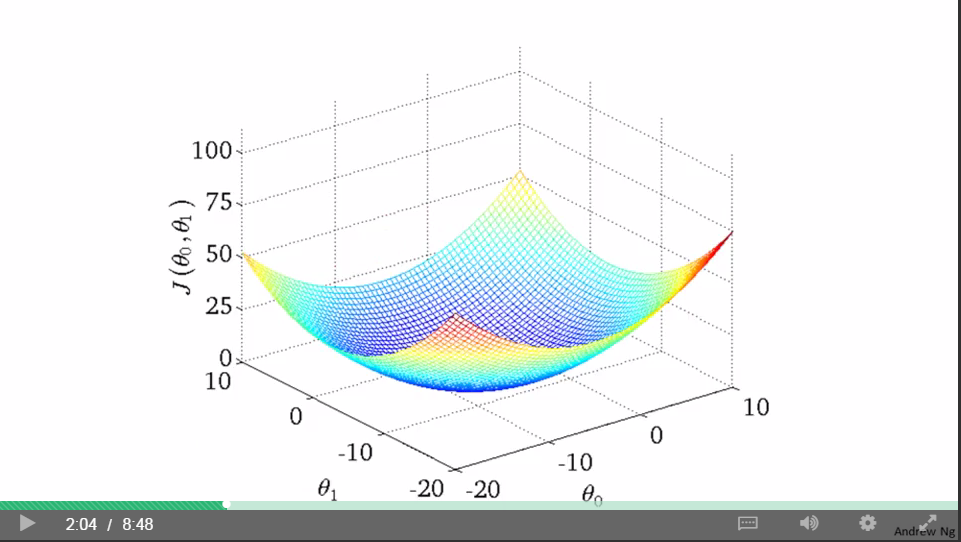
\includegraphics[scale = .5]{1a}
\centering
\caption{The error function is shaped like a hyperplane}
\end{figure}

\begin{figure}[h!]
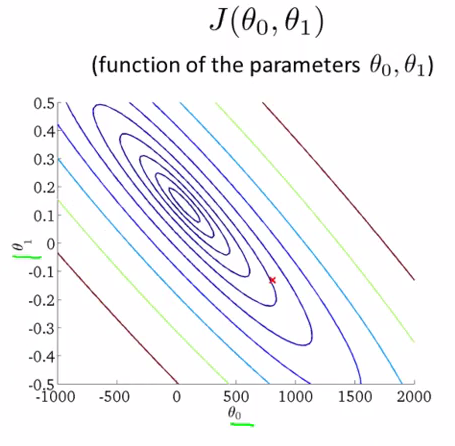
\includegraphics[scale = .75]{1b}
\centering
\caption{Cross sections of the error function}
\end{figure}

\pagebreak

Iteratively, the supervised learning algorithm will try different values for $\Theta_0$ and $\Theta_1$ until it gets to the minimum (represented by the center of these ellipses).



\section{Expanding on One-Variable Regression}
	
For a given data point 
	
	\begin{figure}
		\caption{Dummy figure}
	\end{figure}

	
	\begin{lstlisting}
	# comment
	import pandas as pd
	df = pd.DataFrame()
	one = 100
	string = 'This is a string'
	\end{lstlisting}





\newpage \begin{appendix} \listoffigures \listoftables \end{appendix}
\end{document}